\chapter{Introduction}\label{ch:introduction}

\section{Background and Motivation}
Modern payment platforms process millions of transactions daily, each subject to complex validation rules that protect customers, reduce operational risk, and ensure regulatory compliance. At Deutsche Bank's eBridge-EU system, these validation rules span from simple field validations (mandatory characters, allowed value sets) to intricate domain-specific constraints (country-specific limits, routing conditions, SWIFT/ISO message-format requirements). With hundreds of rules evolving continuously across distributed teams and systems, developers and quality assurance teams face a critical challenge: quickly finding and understanding the exact rules relevant to their current task.

Traditional keyword search fails this use case. Rules are described inconsistently across teams, terminology overlaps, and natural language queries rarely match the exact vocabulary in rule documentation. A developer asking about ``EUR cross-border limits'' might miss rules titled ``SEPA maximum amount validation'' despite their relevance. Moreover, rule data is often scattered across multiple systems, with inconsistent formats and outdated versions. Simultaneously, banking environments impose strict architectural constraints: no external API calls, limited infrastructure dependencies, and complete audit trails for all data access.

\section{Problem Statement}
\textbf{Goal.} Given a user query about a validation rule (e.g., ``EUR cross-border limit'' or ``party agent checks for DE''), the system should:
\begin{enumerate}[leftmargin=*,itemsep=2pt,topsep=2pt]
 \item return a short, ranked list of relevant rules drawn from a \emph{single, standardized CSV corpus};
 \item display all available rule information (codes, tags, language variants, implementation code) and a short, factual explanation grounded in the stored fields;
 \item maintain sub-second response time for typical searches while operating within enterprise infrastructure constraints.
\end{enumerate}

\section{Approach Overview}
This thesis presents a retrieval-augmented generation system that addresses these challenges through a hybrid retrieval architecture. The system combines three complementary signals—lexical matching, fuzzy string similarity, and semantic embeddings—with configurable weights optimized through empirical evaluation. The architecture follows a monolithic design pattern where all components operate within a single process, simplifying deployment and audit compliance.

The key innovation lies in comprehensive data standardization coupled with offline enrichment. Scattered rule data from multiple sources was consolidated into a single CSV corpus with uniform field definitions. Large language models were employed during corpus preparation to generate enhanced descriptions used primarily for embedding generation, ensuring semantic search capabilities without runtime model dependencies. This separation of offline enrichment from online retrieval ensures deterministic, auditable search results.

\section{Corpus and Fields}
Each row in the standardized CSV represents one validation rule, consolidated from distributed sources and cleaned to ensure consistency:
\begin{itemize}[leftmargin=*,itemsep=2pt,topsep=2pt]
 \item \textbf{Identifiers}: \textit{Rule ID, Rule Name} (deduplicated across sources).
 \item \textbf{Business descriptions}: \textit{English Description, German Description} (standardized terminology).
 \item \textbf{Error codes}: \textit{BANSTA Error Code, ISO Error Code} (validated against official registries).
 \item \textbf{LLM-enriched text}: \textit{LLM Generated Description} (created offline, used primarily for embedding generation).
 \item \textbf{Search fields}: \textit{Keywords} (curated terms), \textit{Tags} (Rule Type, Country, Business Type, Party Agent).
 \item \textbf{Metadata}: \textit{Relevance} (a rule-level score in $[0,1]$), \textit{Embedding} (JSON string with 1024 floats), \textit{Versioning}, \textit{Date}.
 \item \textbf{Implementation}: \textit{Rule Code} (the actual validation rule implementation).
\end{itemize}
Embeddings are produced with \texttt{UAE-Large-V1} \cite{uae2023large} (1024 dimensions, mean pooling), L2-normalized, and stored as JSON strings. The bilingual fields (EN/DE) support business users across teams while keeping a single source of truth. This standardization process resolved inconsistencies in naming conventions, merged duplicate rules, and established canonical representations for all fields.

\clearpage
\section{System Overview}
The monolithic Dash application implements a complete RAG pipeline with minimal dependencies and efficient startup initialization:

\begin{figure}[H]
\centering
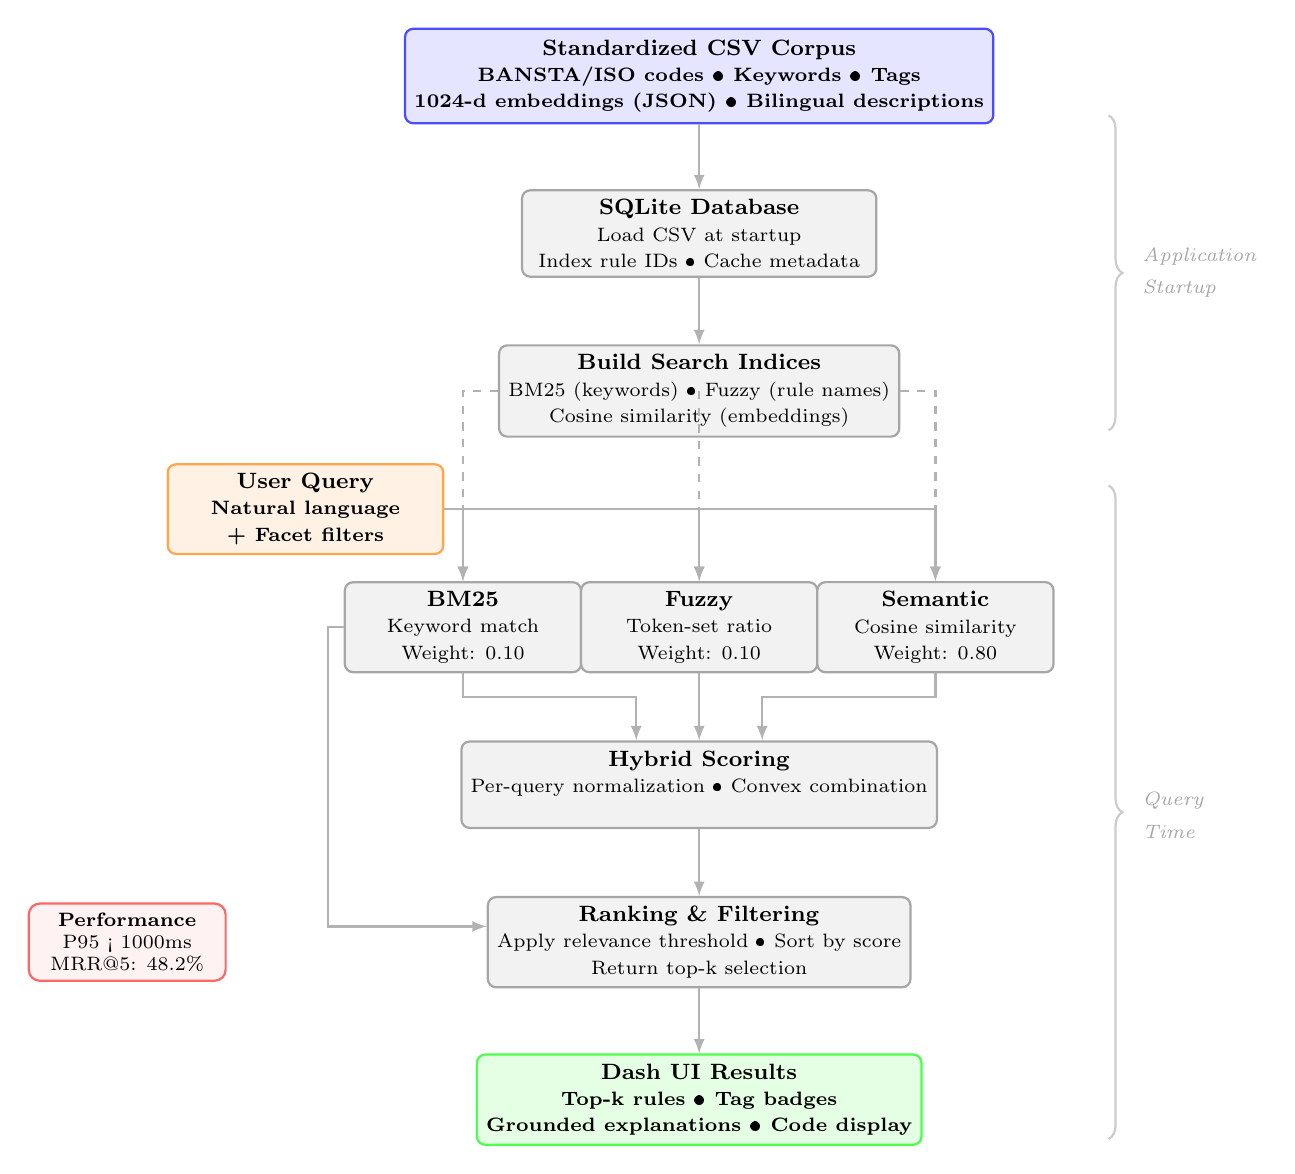
\begin{tikzpicture}[
>=latex,
thick,
font=\footnotesize,
% Node styles
datanode/.style={
  draw=blue!70, 
  fill=blue!10, 
  rounded corners=3pt, 
  minimum width=5cm, 
  minimum height=1.2cm, 
  align=center,
  font=\footnotesize\bfseries
},
processnode/.style={
  draw=gray!70, 
  fill=gray!10, 
  rounded corners=3pt, 
  minimum width=4.5cm, 
  minimum height=1cm, 
  align=center,
  font=\footnotesize
},
querynode/.style={
  draw=orange!70, 
  fill=orange!10, 
  rounded corners=3pt, 
  minimum width=3.5cm, 
  minimum height=0.9cm, 
  align=center,
  font=\footnotesize\bfseries
},
resultnode/.style={
  draw=green!70, 
  fill=green!10, 
  rounded corners=3pt, 
  minimum width=4.5cm, 
  minimum height=1cm, 
  align=center,
  font=\footnotesize\bfseries
},
arrow/.style={->, thick, draw=gray!60},
dashedarrow/.style={->, thick, draw=gray!60, dashed},
label/.style={font=\scriptsize, text=gray!70}
]

% Main vertical flow
\node[datanode] (csv) at (0,0) {
\textbf{Standardized CSV Corpus}\\
\scriptsize BANSTA/ISO codes • Keywords • Tags\\
\scriptsize 1024-d embeddings (JSON) • Bilingual descriptions
};

\node[processnode] (sqlite) at (0,-2) {
\textbf{SQLite Database}\\
\scriptsize Load CSV at startup\\
\scriptsize Index rule IDs • Cache metadata
};

\node[processnode] (indices) at (0,-4) {
\textbf{Build Search Indices}\\
\scriptsize BM25 (keywords) • Fuzzy (rule names)\\
\scriptsize Cosine similarity (embeddings)
};

% User query enters from left
\node[querynode] (query) at (-5,-5.5) {
\textbf{User Query}\\
\scriptsize Natural language\\
\scriptsize + Facet filters
};

% Three parallel retrieval paths
\node[processnode, minimum width=3cm] (bm25) at (-3,-7) {
\textbf{BM25}\\
\scriptsize Keyword match\\
\scriptsize Weight: 0.10
};

\node[processnode, minimum width=3cm] (fuzzy) at (0,-7) {
\textbf{Fuzzy}\\
\scriptsize Token-set ratio\\
\scriptsize Weight: 0.10
};

\node[processnode, minimum width=3cm] (semantic) at (3,-7) {
\textbf{Semantic}\\
\scriptsize Cosine similarity\\
\scriptsize Weight: 0.80
};

% Scoring and ranking
\node[processnode, minimum width=5cm] (hybrid) at (0,-9) {
\textbf{Hybrid Scoring}\\
\scriptsize Per-query normalization • Convex combination\\
};

\node[processnode, minimum width=5cm] (rank) at (0,-11) {
\textbf{Ranking \& Filtering}\\
\scriptsize Apply relevance threshold • Sort by score\\
\scriptsize Return top-k selection
};

\node[resultnode] (results) at (0,-13) {
\textbf{Dash UI Results}\\
\scriptsize Top-k rules • Tag badges\\
\scriptsize Grounded explanations • Code display
};

% Arrows for main flow
\draw[arrow] (csv) -- (sqlite);
\draw[arrow] (sqlite) -- (indices);

% Query flows to all three retrievers
\draw[arrow] (query) -| (bm25);
\draw[arrow] (query) -| (fuzzy);
\draw[arrow] (query) -| (semantic);

% Indices connection (dashed to show pre-built)
\draw[dashedarrow] (indices) -| (bm25.north);
\draw[dashedarrow] (indices) -| (fuzzy.north);
\draw[dashedarrow] (indices) -| (semantic.north);

% Convergence to hybrid scoring
\draw[arrow] (bm25.south) -- ++(0,-0.3) -| ([xshift=-0.8cm]hybrid.north);
\draw[arrow] (fuzzy.south) -- (hybrid.north);
\draw[arrow] (semantic.south) -- ++(0,-0.3) -| ([xshift=0.8cm]hybrid.north);

% Add direct path from BM25 to Ranking (for Keyword mode)
\draw[arrow] (bm25.west) -- ++(-0.2,0) |- ([yshift=0.2cm]rank.west);

% Final flow
\draw[arrow] (hybrid) -- (rank);
\draw[arrow] (rank) -- (results);

% Timing annotations
\node[label, anchor=west] at (5.5,-2.3) {\textit{Application}};
\node[label, anchor=west] at (5.5,-2.7) {\textit{Startup}};
\draw[gray!40, thick, decorate, decoration={brace, amplitude=5pt}] 
(5.2,-0.5) -- (5.2,-4.5);

\node[label, anchor=west] at (5.5,-9.2) {\textit{Query}};
\node[label, anchor=west] at (5.5,-9.6) {\textit{Time}};
\draw[gray!40, thick, decorate, decoration={brace, amplitude=5pt}] 
(5.2,-5.2) -- (5.2,-13.5);

% Performance annotation
\node[draw=red!60, fill=red!5, rounded corners, anchor=east, 
    font=\scriptsize, align=center, minimum width=2.5cm] 
    at (-6,-11) {
\textbf{Performance}\\
P95 < 1000ms\\
MRR@5: 48.2\%
};

\end{tikzpicture}
\caption{Monolithic RAG architecture with vertical data flow. The system follows a clear pipeline from data ingestion at startup through query-time retrieval and ranking. Three retrieval signals (BM25, Fuzzy, Semantic) operate in parallel with empirically tuned weights from LOOCV evaluation. The relevance threshold filters low-confidence results regardless of retrieval mode. All components run in-process within a single Dash application.}\label{fig:intro-architecture}
\end{figure}

\begin{itemize}[leftmargin=*,itemsep=2pt,topsep=2pt]
 \item \textbf{Data Layer}: CSV ingestion into SQLite at startup, JSON embedding parsing into numpy arrays, L2 normalization, in-memory caching of all indices. All LLM processing (description generation, keyword extraction) occurs offline during corpus preparation.
 \item \textbf{Retrieval Layer}: Three parallel retrievers initialized at startup—BM25 index \cite{robertson2009bm25} over keywords, fuzzy matcher \cite{fuzzywuzzy2011} on rule names, and semantic search via cosine similarity on the embedding matrix. 
 \item \textbf{Ranking Layer}: Per-query score normalization, convex combination with tuned weights (0.10/0.10/0.80), followed by relevance threshold filtering at $\tau=0.30$ to exclude low-confidence results.
 \item \textbf{UI Layer}: Dash components for mode selection (Keyword/Hybrid), faceted filtering, ranked result cards displaying all available rule information including code implementation with tag badges, and grounded explanation panels rendered from stored fields.
\end{itemize}

\section{Retrieval Modes and Scoring}

The system internally maintains three retrieval mechanisms (BM25, fuzzy matching, and semantic search) but exposes only two modes through the user interface: \textbf{Keyword mode}, which uses BM25 scoring alone, and \textbf{Hybrid mode}, which combines all three signals with learned weights. This design balances simplicity for users with comprehensive retrieval coverage.

\paragraph{Keyword mode (BM25).} 
We index the \emph{Keywords} field at startup and compute BM25 scores for queries. This mode is deterministic and fast, performing well when query vocabulary matches the curated keywords.

\paragraph{Hybrid mode (three signals).} 
For each candidate rule $r$ with keywords $K(r)$ and LLM description $D(r)$:
\[
s_{\text{kw}} = \mathrm{BM25}(q, K(r)),\quad s_{\text{fuzzy}} = \tfrac{1}{100}\,\mathrm{TokenSetRatio}(q, \mathrm{name}(r)),\quad s_{\text{sem}} = \cos\!\big(\phi(q), \psi(D(r))\big),
\]
where $\phi$ and $\psi$ are \texttt{UAE-Large-V1} encoders (1024-d, mean pooling). Scores are min–max normalized per query across the candidate pool to $[0,1]$. 

The final score is a convex combination with weights empirically tuned via Leave-One-Out Cross-Validation (LOOCV):
\[
s_{\text{hybrid}} = 0.10\,\widehat{s}_{\text{kw}} + 0.10\,\widehat{s}_{\text{fuzzy}} + 0.80\,\widehat{s}_{\text{sem}}
\]

We then apply a relevance threshold to filter low-confidence results across all modes:
\[
\boxed{ \; s_{\text{final}} = \begin{cases}
s_{\text{mode}} & \text{if } s_{\text{mode}} \ge \tau \\
0 & \text{otherwise}
\end{cases}
\quad \text{with} \quad \tau = 0.30 \; }
\]
where $s_{\text{mode}}$ is either $s_{\text{kw}}$ for Keyword mode or $s_{\text{hybrid}}$ for Hybrid mode. These weights maximize Mean Reciprocal Rank at 5 (MRR@5) on our evaluation dataset (30 manually annotated query-rule pairs), improving from 43.4\% (initial weights) to 48.2\% (tuned weights). While the evaluation set is limited in size, each annotation was carefully validated to ensure high quality.

\paragraph{Why this design works.} 
The hybrid approach balances precision and coverage:
\begin{itemize}[leftmargin=*,itemsep=2pt,topsep=2pt]
 \item BM25 anchors results in the curated vocabulary from the standardized corpus.
 \item Fuzzy matching tolerates minor spelling or tokenization differences in rule names.
 \item Semantic similarity captures meaning when wording diverges but intent remains aligned.
 \item The relevance threshold ($\tau=0.30$) filters low-confidence results regardless of retrieval mode.
 \item SQLite provides efficient filtering and sorting without external database dependencies.
 \item Pre-built indices at startup eliminate query-time index construction overhead.
\end{itemize}

\section{Operational Constraints and Non-Goals}
\paragraph{Constraints.} The system is designed for a regulated banking environment with stringent security and compliance requirements:
\begin{itemize}[leftmargin=*,itemsep=2pt,topsep=2pt]
 \item \textbf{Banking-approved technology stack}. The system uses only established, auditable technologies that meet financial sector security standards. Dense similarity computation relies on \texttt{scikit-learn}'s \texttt{cosine\_similarity} \cite{pedregosa2011sklearn} with in-memory vectors parsed from the CSV's JSON embedding field at startup.
 \item \textbf{Latency requirement}. P95 latency must remain under 1000ms for top-k retrieval on the full corpus (${\sim}10^3$ rules), measured end-to-end from query submission to UI render.
 \item \textbf{Single-file deployment}. The entire rule corpus, including embeddings, must remain in a single CSV file for audit trail, version control, and regulatory compliance purposes.
\end{itemize}
\paragraph{Non-goals.} The system does not execute validation rules, analyze source code semantics, or validate runtime behavior. Its sole purpose is \emph{information retrieval} and \emph{grounded explanation} over the standardized tabular rule corpus.

\section{Research Questions}
\begin{description}[leftmargin=!,labelwidth=2.5cm,itemsep=2pt,topsep=2pt]
 \item[RQ1:] What is the optimal weight configuration for hybrid retrieval, and how much does it improve MRR@5 over individual signals?
 \item[RQ2:] How robust is performance to weight perturbations, and what is the contribution of each signal in ablation studies?
 \item[RQ3:] Does the relevance threshold ($\tau{=}0.30$) effectively filter noise while preserving relevant results?
 \item[RQ4:] Can the system maintain P95 latency under 1000ms while serving concurrent users in a production Dash deployment?
\end{description}

\section{Contributions}
\begin{enumerate}[leftmargin=*,itemsep=2pt,topsep=2pt]
 \item A production-ready, monolithic RAG system for validation rule retrieval that operates within banking infrastructure constraints using only auditable, established technologies.
 \item A comprehensive data standardization pipeline that consolidated distributed, inconsistent rule sources into a single, clean CSV corpus with uniform field definitions and validated error codes.
 \item An empirically optimized hybrid retrieval approach with LOOCV-tuned weights (semantic 0.80, BM25 0.10, fuzzy 0.10) and relevance threshold filtering ($\tau{=}0.30$).
 \item A complete full-stack implementation in Dash with efficient startup initialization—SQLite ingestion and index building—demonstrating that sophisticated NLP capabilities can be delivered through simple, auditable architectures.
 \item Rigorous evaluation using Leave-One-Out Cross-Validation showing 48.2\% MRR@5, with detailed ablation studies and sensitivity analyses confirming robustness.
 \item A CSV-first data architecture that stores 1024-dimensional embeddings as JSON strings, enabling single-file deployment while maintaining sub-second query performance through in-memory indexing.
\end{enumerate}

\section{Thesis Structure}

The remainder of this thesis is organized into seven chapters:

\textbf{Chapter~2: Related Work} positions this research within the existing literature on hybrid retrieval systems and rule discovery in financial compliance contexts. The chapter identifies critical gaps in current approaches, particularly the lack of unified retrieval systems for multilingual regulatory corpora.

\textbf{Chapter~3: Fundamentals} establishes the theoretical foundation of information retrieval techniques employed in this work. It covers BM25 scoring for sparse keyword matching, fuzzy string matching algorithms for approximate rule name search, dense embeddings using UAE-Large-V1 for semantic similarity, and the Retrieval-Augmented Generation (RAG) architectural pattern.

\textbf{Chapter~4: Corpus Analysis} provides a detailed examination of the standardized rule corpus post-consolidation. Analysis includes field completeness metrics, tag distribution patterns, embedding quality assessment, and identification of data challenges such as missing translations and sparse metadata.

\textbf{Chapter~5: System Design} presents the architectural decisions underlying the retrieval system. Core components include the hybrid scoring function with empirically-tuned weights, per-query score normalization strategy, SQLite database schema for efficient indexing, and the monolithic Dash application structure.

\textbf{Chapter~6: Implementation} details the Python codebase organization, startup initialization sequence, and engineering choices enabling efficient in-memory operation. The chapter emphasizes the deliberate avoidance of external dependencies in favor of self-contained functionality.

\textbf{Chapter~7: Evaluation} reports comprehensive experimental results. Methodologies include Leave-One-Out Cross-Validation (LOOCV) for hyperparameter tuning, ablation studies isolating component contributions, and sensitivity analyses examining system robustness to parameter variations.

\textbf{Chapter~8: Conclusion} synthesizes the contributions, acknowledges limitations of the CSV-first approach, and proposes future research directions including graded relevance annotations, neural re-ranking models, and conversational interface development.
